        %%******************************************%%
        %%                                          %%
        %%        Modello di tesi di laurea         %%
        %%            di Andrea Giraldin            %%
        %%                                          %%
        %%             2 novembre 2012              %%
        %%                                          %%
        %%******************************************%%

% !TEX spellcheck = it-IT     controllo ortografico italiano per l'editor

% PDF/A filecontents
\RequirePackage{filecontents}
\begin{filecontents*}{\jobname.xmpdata}
  \Title{Analisi, progettazione e sviluppo del backend di un'applicazione web per la gestione di eventi}
  \Author{Alberto Lazari}
  \Language{it-IT}
  \Subject{Moku S.r.l. sta sviluppando per conto di un'importante realtà del territorio un'applicazione web per la gestione di eventi fisici, online e ibridi. L'obiettivo dell'applicazione è quello di essere un software as a service multi tenant che possa soddisfare le esigenze di diversi tipi di organizzatori di eventi, siano essi fiere, convegni o corsi di formazione.}
  \Keywords{Backend \sep Ruby on Rails \sep Videoconferenze \sep Gestione eventi}
\end{filecontents*}

\documentclass[10pt,      % corpo del font principale
               a4paper,   % carta A4
               twoside,   % impagina per fronte-retro
               openright, % inizio capitoli a destra
               english,                 
               italian,                 
               ]{book}    

% Importazione package

\PassOptionsToPackage{table}{xcolor}

% colori PDF/A
\PassOptionsToPackage{dvipsnames}{xcolor}

\usepackage{colorprofiles}

% configurazione PDF/A
% validare in https://www.pdf-online.com/osa/validate.aspx
\usepackage[a-2b,mathxmp]{pdfx}[2018/12/22]

% formule matematiche
%\usepackage{amsmath,amssymb,amsthm}

% codifica dei font:
% NOTA BENE! richiede una distribuzione *completa* di LaTeX
\usepackage[T1]{fontenc}
\usepackage[utf8]{inputenc}

% per scrivere in italiano e in inglese
% l'ultima lingua (l'italiano) risulta predefinita
\usepackage[english, italian]{babel}

\usepackage{bookmark}                   % segnalibri

\usepackage{caption}                    % didascalie

\usepackage{chngpage,calc}              % centra il frontespizio

\usepackage{csquotes}                   % gestisce automaticamente i caratteri (")

\usepackage{emptypage}                  % pagine vuote senza testatina e piede di pagina

\usepackage{epigraph}			              % per le citazioni

\usepackage{eurosym}                    % simbolo dell'euro

%\usepackage{indentfirst}               % rientra il primo paragrafo di ogni sezione

\usepackage{graphicx}                   % immagini

\usepackage{hyperref}                   % collegamenti ipertestuali

\usepackage[binding=5mm]{layaureo}      % margini ottimizzati per l'A4; rilegatura di 5 mm

\usepackage{listings}                   % codici

\usepackage{microtype}                  % microtipografia

\usepackage{mparhack,fixltx2e,relsize}  % finezze tipografiche

\usepackage{nameref}                    % visualizza nome dei riferimenti                                      
\usepackage[font=small]{quoting}        % citazioni

\usepackage{subfig}                     % sottofigure, sottotabelle

\usepackage[italian]{varioref}          % riferimenti completi della pagina

\usepackage{booktabs}                   % tabelle                                       
\usepackage{tabularx}                   % tabelle di larghezza prefissata                                    
\usepackage{longtable}                  % tabelle su più pagine                                        
\usepackage{ltxtable}                   % tabelle su più pagine e adattabili in larghezza

% glossario
% per includerlo nel documento bisogna:
%   1. compilare una prima volta tesi.tex
%   2. eseguire: makeindex -s tesi.ist -t tesi.glg -o tesi.gls tesi.glo
%   3. eseguire: makeindex -s tesi.ist -t tesi.alg -o tesi.acr tesi.acn
%   4. compilare due volte tesi.tex
\usepackage[toc, acronym]{glossaries}

% eccellente pacchetto per la bibliografia
% produce uno stile di citazione autore-anno
% lo stile "numeric-comp" produce riferimenti numerici
% per includerlo nel documento bisogna:
%   1. compilare una prima volta tesi.tex
%   2. eseguire: biber tesi
%   3. compilare ancora tesi.tex
\usepackage[backend=biber,style=verbose-ibid,hyperref,backref]{biblatex}

\usepackage{makecell}

\usepackage[outputdir=build]{minted}
\usemintedstyle{emacs}
\setminted{
  bgcolor=lightgray,
  fontsize=\small,
  tabsize=2,
  breaklines
}

% Environment per il codice
% si utilizza con \begin{code}[lang]{caption}
\makeatletter
\newenvironment{code}[2][ruby]
{
  \VerbatimEnvironment
  \begin{listing}[H]
    \caption{#2}
    \begin{minted}{#1}
}
{
    \end{minted}
  \end{listing}
}
\makeatother

% file con le impostazioni personali
% file contenente le impostazioni della tesi

% Frontespizio

% Autore
\newcommand{\myName}{Alberto Lazari}
\newcommand{\myTitle}{Analisi, progettazione e sviluppo del backend di un'applicazione web per la gestione di eventi}

% Tipo di tesi
\newcommand{\myDegree}{Tesi di laurea}

% Università
\newcommand{\myUni}{Università degli Studi di Padova}

% Facoltà
\newcommand{\myFaculty}{Corso di Laurea in Informatica}

% Dipartimento
\newcommand{\myDepartment}{Dipartimento di Matematica "Tullio Levi-Civita"}

% Titolo del relatore
\newcommand{\profTitle}{Prof.}

% Relatore
\newcommand{\myProf}{Davide Bresolin}

% Luogo
\newcommand{\myLocation}{Padova}

% Anno accademico
\newcommand{\myAA}{2021-2022}

% Data discussione
\newcommand{\myTime}{Luglio 2022}


% Impostazioni di impaginazione
% see: http://wwwcdf.pd.infn.it/AppuntiLinux/a2547.htm

\setlength{\parindent}{14pt}   % larghezza rientro della prima riga
\setlength{\parskip}{0pt}   % distanza tra i paragrafi


% Impostazioni di biblatex
\addbibresource{../bibliografia.bib}
\bibliography{bibliografia} % database di biblatex 

\defbibheading{bibliography} {
    \cleardoublepage
    \phantomsection 
    \addcontentsline{toc}{chapter}{\bibname}
    \chapter*{\bibname\markboth{\bibname}{\bibname}}
}

\setlength\bibitemsep{1.5\itemsep} % spazio tra entry

\DeclareBibliographyCategory{opere}
\DeclareBibliographyCategory{web}

\defbibheading{opere}{\section*{Riferimenti bibliografici}}
\defbibheading{web}{\section*{Siti Web consultati}}


% Impostazioni di caption
\captionsetup{
    tableposition=top,
    figureposition=bottom,
    font=small,
    format=hang,
    labelfont=bf
}

% Impostazioni di graphicx
\graphicspath{{immagini/}} % cartella dove sono riposte le immagini


% Impostazioni di hyperref
\hypersetup{
    %hyperfootnotes=false,
    %pdfpagelabels,
    %draft,	% = elimina tutti i link (utile per stampe in bianco e nero)
    colorlinks=true,
    %linktocpage=true,  % mette i link sui numeri delle pagine
    pdfstartpage=1,
    pdfstartview=,
    % decommenta la riga seguente per avere link in nero (per esempio per la stampa in bianco e nero)
    %colorlinks=false, linktocpage=false, pdfborder={0 0 0}, pdfstartpage=1, pdfstartview=FitV,
    breaklinks=true,
    pdfpagemode=UseNone,
    pageanchor=true,
    pdfpagemode=UseOutlines,
    plainpages=false,
    bookmarksnumbered,
    bookmarksopen=true,
    bookmarksopenlevel=1,
    hypertexnames=true,
    pdfhighlight=/O,
    %nesting=true,
    %frenchlinks,
    urlcolor=webbrown,
    linkcolor=RoyalBlue,
    citecolor=webgreen,
    %pagecolor=RoyalBlue,
    urlcolor=Black, linkcolor=Black, citecolor=Black, %pagecolor=Black,
}

% Impostazioni di itemize
\renewcommand{\labelitemi}{$\circ$}
%\renewcommand{\labelitemi}{$\ast$}
%\renewcommand{\labelitemi}{$\bullet$}
%\renewcommand{\labelitemii}{$\cdot$}
%\renewcommand{\labelitemiii}{$\diamond$}
%\renewcommand{\labelitemiv}{$\ast$}


% Impostazioni di listings
\lstset{
    language=[LaTeX]Tex,%C++,
    keywordstyle=\color{RoyalBlue}, %\bfseries,
    basicstyle=\small\ttfamily,
    %identifierstyle=\color{NavyBlue},
    commentstyle=\color{Green}\ttfamily,
    stringstyle=\rmfamily,
    numbers=none, %left,%
    numberstyle=\scriptsize, %\tiny
    stepnumber=5,
    numbersep=8pt,
    showstringspaces=false,
    breaklines=true,
    frameround=ftff,
    frame=single
} 


% Impostazioni di xcolor
\definecolor{webgreen}{rgb}{0,.5,0}
\definecolor{webbrown}{rgb}{.6,0,0}


% Altro

\newcommand{\omissis}{[\dots\negthinspace]} % produce [...]

% eccezioni all'algoritmo di sillabazione
\hyphenation
{
    ma-cro-istru-zio-ne
}

\newcommand{\sectionname}{sezione}
\addto\captionsitalian{\renewcommand{\figurename}{Figura}
                       \renewcommand{\tablename}{Tabella}}

\newcommand{\glsfirstoccur}{\ap{{[g]}}}

\newcommand{\intro}[1]{\emph{#1}}

% Environment per ``rischi''
\newcounter{riskcounter}                % define a counter
\setcounter{riskcounter}{0}             % set the counter to some initial value

%%%% Parameters
% #1: Title
\newenvironment{risk}[1]{
    \refstepcounter{riskcounter}        % increment counter
    \par \noindent                      % start new paragraph
    \textbf{\arabic{riskcounter}. #1}   % display the title before the 
                                        % content of the environment is displayed 
}{
    \par\medskip
}

\newcommand{\riskname}{Rischio}

\newcommand{\riskdescription}[1]{\textbf{\\Descrizione:} #1.}

\newcommand{\risksolution}[1]{\textbf{\\Soluzione:} #1.}

% Environment per ``use case''
\newcounter{usecasecounter}             % define a counter
\setcounter{usecasecounter}{0}          % set the counter to some initial value

%%%% Parameters
% #1: ID
% #2: Nome
\newenvironment{usecase}[2]{
    \renewcommand{\theusecasecounter}{\usecasename #1}  % this is where the display of 
                                                        % the counter is overwritten/modified
    \refstepcounter{usecasecounter}             % increment counter
    \vspace{10pt}
    \par \noindent                              % start new paragraph
    {\large \textbf{\usecasename #1: #2}}       % display the title before the 
                                                % content of the environment is displayed 
    \medskip
}{
    \medskip
}

\newcommand{\usecasename}{UC}

\newcommand{\usecaseactors}[1]{\textbf{\\Attori Principali:} #1. \vspace{4pt}}
\newcommand{\usecasepre}[1]{\textbf{\\Precondizioni:} #1. \vspace{4pt}}
\newcommand{\usecasedesc}[1]{\textbf{\\Descrizione:} #1. \vspace{4pt}}
\newcommand{\usecasepost}[1]{\textbf{\\Postcondizioni:} #1. \vspace{4pt}}
\newcommand{\usecasealt}[1]{\textbf{\\Scenario Alternativo:} #1. \vspace{4pt}}

% Environment per ``namespace description''

\newenvironment{namespacedesc}{
    \vspace{10pt}
    \par \noindent                              % start new paragraph
    \begin{description} 
}{
    \end{description}
    \medskip
}

\newcommand{\classdesc}[2]{\item[\textbf{#1:}] #2}


\begin{document}
  % Materiale iniziale
  \frontmatter
  % !TEX encoding = UTF-8
% !TEX TS-program = pdflatex
% !TEX root = ../tesi.tex

%**************************************************************
% Frontespizio 
%**************************************************************
\begin{titlepage}

\begin{center}

\begin{LARGE}
\textbf{\myUni}\\
\end{LARGE}

\vspace{10pt}

\begin{Large}
\textsc{\myDepartment}\\
\end{Large}

\vspace{10pt}

\begin{large}
\textsc{\myFaculty}\\
\end{large}

\vspace{50pt}
\begin{figure}[htbp]
\begin{center}

\includegraphics[height=6cm]{logo-unipd}
\end{center}
\end{figure}
\vspace{15pt}

\begin{LARGE}
\begin{center}
\textbf{\myTitle}\\
\end{center}
\end{LARGE}

\vspace{10pt}

\begin{large}
\textsl{\myDegree}\\
\end{large}

\vspace{30pt}

\begin{large}
\begin{flushleft}
\textit{Relatore} \\
\vspace{5pt}
\profTitle \myProf
\end{flushleft}

\vspace{-43pt}

\begin{flushright}
\textit{Laureando} \\
\vspace{5pt}
\myName
\end{flushright}
\end{large}

\vspace{70pt}

\line(1, 0){338} \\
\begin{normalsize}
\textsc{Anno Accademico \myAA}
\end{normalsize}

\end{center}
\end{titlepage} 
  % !TEX encoding = UTF-8
% !TEX TS-program = pdflatex
% !TEX root = ../tesi.tex

%**************************************************************
% Colophon
%**************************************************************
\clearpage
\phantomsection
\thispagestyle{empty}

\hfill

\vfill

\noindent\myName: \textit{\myTitle,}
\myDegree,
\textcopyright\ \myTime.
  % !TEX encoding = UTF-8
% !TEX TS-program = pdflatex
% !TEX root = ../tesi.tex

%**************************************************************
% Sommario
%**************************************************************
\cleardoublepage
\phantomsection
\pdfbookmark{Sommario}{Sommario}
\begingroup
\let\clearpage\relax
\let\cleardoublepage\relax
\let\cleardoublepage\relax

\chapter*{Sommario}

Il presente documento descrive il lavoro svolto durante il periodo di stage, della durata di circa trecento ore, dal laureando Pinco Pallino presso l'azienda Azienda S.p.A.
Gli obbiettivi da raggiungere erano molteplici.\\
In primo luogo era richiesto lo sviluppo di ...
In secondo luogo era richiesta l'implementazione di un ... 
Tale framework permette di registrare gli eventi di un controllore programmabile, quali segnali applicati 
Terzo ed ultimo obbiettivo era l'integrazione ...

%\vfill
%
%\selectlanguage{english}
%\pdfbookmark{Abstract}{Abstract}
%\chapter*{Abstract}
%
%\selectlanguage{italian}

\endgroup			

\vfill


  % !TEX encoding = UTF-8
% !TEX TS-program = pdflatex
% !TEX root = ../tesi.tex

%**************************************************************
% Ringraziamenti
%**************************************************************
\cleardoublepage
\phantomsection
\pdfbookmark{Ringraziamenti}{ringraziamenti}

\begin{flushright}{
	\slshape    
	``Life is really simple, but we insist on making it complicated''} \\ 
	\medskip
    --- Confucius
\end{flushright}


\bigskip

\begingroup
\let\clearpage\relax
\let\cleardoublepage\relax
\let\cleardoublepage\relax

\chapter*{Ringraziamenti}

\noindent \textit{Innanzitutto, vorrei esprimere la mia gratitudine al Prof. NomeDelProfessore, relatore della mia tesi, per l'aiuto e il sostegno fornitomi durante la stesura del lavoro.}\\

\noindent \textit{Desidero ringraziare con affetto i miei genitori per il sostegno, il grande aiuto e per essermi stati vicini in ogni momento durante gli anni di studio.}\\

\noindent \textit{Ho desiderio di ringraziare poi i miei amici per tutti i bellissimi anni passati insieme e le mille avventure vissute.}\\
\bigskip

\noindent\textit{\myLocation, \myTime}
\hfill \myName

\endgroup


  % !TEX encoding = UTF-8
% !TEX TS-program = pdflatex
% !TEX root = ../tesi.tex

%**************************************************************
% Indici
%**************************************************************
\cleardoublepage
\pdfbookmark{\contentsname}{tableofcontents}
\setcounter{tocdepth}{2}
\tableofcontents
%\markboth{\contentsname}{\contentsname} 
\clearpage

\begingroup 
    \let\clearpage\relax
    \let\cleardoublepage\relax
    \let\cleardoublepage\relax
    %*******************************************************
    % Elenco delle figure
    %*******************************************************    
    \phantomsection
    \pdfbookmark{\listfigurename}{lof}
    \listoffigures

    \vspace*{8ex}

    %*******************************************************
    % Elenco delle tabelle
    %*******************************************************
    \phantomsection
    \pdfbookmark{\listtablename}{lot}
    \listoftables
        
    \vspace*{8ex}
\endgroup

\cleardoublepage

  \cleardoublepage

  % Capitoli
  \mainmatter

  \chapter{L'azienda}
  \label{cap:azienda}   
  \section{Descrizione generale}

\begin{center}
	
\includegraphics[height = 4cm]{moku-logo}
\end{center}

\noindent Moku S.r.l.\ è una start-up nata nel 2013 all'interno di un progetto supportato da H-Farm. Dopo aver abbandonato il progetto si è dedicata allo sviluppo software su commissione e consulenza, per poi allontanarsi definitivamente da H-Farm a settembre 2021, muovendo la sua sede dalla \emph{farm} a Roncade a quella attuale di Treviso. \\
L'azienda è in continua espansione e conta circa 20 dipendenti, la maggior parte con età inferiore ai 30 anni. Questo contribuisce a mantenere l'ambiente di lavoro stimolante e accogliente per tutti, permettendo di includere i diversi studenti che ogni anno svolgono il loro stage presso l'azienda. Per questi vengono attivate proposte di progetto per i ruoli di sviluppatore backend, sviluppatore frontend e sviluppatore mobile, all'interno di team interni che lavorano a progetti reali commissionati all'azienda.

\section{Modello di sviluppo}
I progetti di Moku seguono un modello di sviluppo \emph{agile}, con metodologie basate su \emph{Scrum} \footcite{site:scrum-guide}, un framework pensato per team di sviluppo sotware di piccole dimensioni (non più di dieci membri).
Il lavoro viene suddiviso in \emph{sprint}, intervalli temporali della durata di due settimane. Ogni \emph{sprint} è preceduto da una riunione di pianificazione degli obiettivi, espressi sotto forma di \emph{user stories}, che esprimono le funzionalità del software da implementare, scritte in un lunguaggio naturale dal punto di vista dell'utente. Uno \emph{sprint} termina con la \emph{sprint review} associata, una riunione con il cliente che ha l'obiettivo di mostrare l'incremento prodotto nel software, attraverso dimostrazioni del funzionamento del software stesso.

Il team a cui viene affidato lo sviluppo di un progetto è composto da diverse figure professionali, tra cui un \emph{project manager}, il cui compito è coordinare il lavoro tra gli altri componenti e definire le \emph{user stories} da inserire nel \emph{backlog} degli \emph{sptint}, oltre a gestire la pianificazione dello \emph{sprint} stesso. Per condividere lo stato del lavoro di ogni componente, descrivere gli obiettivi del giorno e far emergere eventuali problemi sorti durante lo sviluppo, il team si riunisce nello \emph{stand-up meeting} all'inizio di ogni giornata lavorativa, una riunione della durata di circa 15 minuti.

La metodologia adottata permette di avere una comunicazione regolare ed efficace tra il team di sviluppo e il cliente, che porta a una definizione più semplice e precisa dei requisiti che il prodotto deve rispettare e a una comprensione immediata e chiara dell'avanzamento dello sviluppo da parte del cliente, attraverso le dimostrazioni pratiche effettuate nel contesto delle \emph{sprint review}.


  \chapter{Descrizione dello stage}
  \label{cap:descrizione-stage}
  \section{Introduzione al progetto}
\intro{Storia del progetto prima del mio arrivo, azienda che ha commissionato il progetto, descrizione dello scopo della piattaforma e del suo funzionamento, motivazioni alla base della scelta di riscrittura del backend.}


\section{Requisiti}
I requisiti dello stage riportati nel piano di lavoro sono i seguenti, categorizzati per importanza:

\paragraph{Obbligatori} Requisiti primari, necessari per una buona riuscita dello stage:
\begin{itemize}
	\item gestione e pianificazione del progetto attraverso kanban board condivisa;
	\item analisi dei flussi attuali e delle API richieste;
	\item progettazione ed implementazione dei modelli e dei controller, a partire dai requisiti raccolti;
	\item analisi ed integrazione Zoom, GoToWebinar, Webex.
\end{itemize}

\paragraph{Desiderabili} Non necessari, ma che contribuiscono alla completezza del prodotto, se rispettati:
\begin{itemize}
	\item coordinamento con il cliente finale;
	\item integrazione team;
	\item integrazione stampante biglietti;
	\item suite di testing del software prodotto;
	\item documentazione completa.
\end{itemize}

\paragraph{Opzionali} Che portano del valore aggiunto al progetto:
\begin{itemize}
	\item ulteriori modifiche all'applicazione che esulano da quando riportato in questo documento.
\end{itemize}


\section{Pianificazione}
\intro{Divisione settimanale del lavoro dal piano di lavoro, incluse correzioni.}


\section{Tecnologie utilizzate}
\intro{Descrizione della configurazione del framework Ruby on Rails utilizzata: librerie utilizzate, Postgres, AWS, API REST.}


  \chapter{Analisi e refactor dei modelli}
  \label{cap:modelli}
  \section{Introduzione}
La prima attività che ho dovuto svolgere è stata la definizione dei modelli del nuovo backend. Purtroppo l'architettura già presente nel vecchio backend, soprattutto lato database, aveva diversi difetti e andava rivista interamente, quindi è stato necessario partire da un'analisi di quanto già fatto, per capire se fosse necessario effettuare del refactor nella struttura dei dati. In molti casi le entità contenevano molti attributi superflui o non adatti ad essere associati alla specifica entità, perché più adatti ad essere associati attraverso una relazione a un'altra entità.\ Le decisioni sono state prese anche basandosi sull'analisi dei requisiti già fatta precedentemente al mio arrivo. Questa è stata tradotta in \emph{user stories}, che hanno guidato la successiva fase di codifica.

L'architettura per il nuovo backend è quella inferita dalle convenzioni di Rails, soprattutto a causa dell'applicazione del pattern Active Record.\ Essendo le classi dei modelli dell'applicazione strettamente legate alle entità presenti nel database, la loro progettazione è stata fatta proseguire parallelamente, al punto che in molti casi è possibile riferirsi interscambiabilmente a attributi di un'entità o del modello associato. Per riferirsi a modelli ed entità verranno seguite le convenzioni di Rails: i nomi dei modelli sono scritti al singolare in \verb|PascalCase|, mentre quelli delle entità sono al plurale in \verb|snake_case|, ad esempio al modello \verb|EventParticipation| è associata l'entità \verb|event_participations|.

In questo capitolo vengono riportati i cambiamenti e le scelte più significative che sono state fatte durante questa fase, che hanno portato alla produzione del diagramma ER completo dell'applicazione, riportato nell'appendice \ref{cap:ER}.

\section{Modifiche significative effettuate}
\subsection{Utenti} \label{modelli:utenti}
La prima tabella analizzata è stata quella degli utenti. Nella versione precedente le informazioni relative al modello degli utenti erano divise in tre entità:
\begin{itemize}
	\item \verb|e_users|: conteneva i dettagli principali degli utenti, come nome, cognome e email, i campi per la gestione dell'autenticazione e altri, che però erano inutilizzati;
	\item \verb|e_partecipants|: era dedicata agli utenti partecipanti. Conteneva un sottoinsieme dei campi di \verb|e_users|:
	\begin{itemize}
		\item \verb|companyId|,
		\item \verb|firstName|,
		\item \verb|lastName|,
		\item \verb|email|,
		\item \verb|phone|,
		\item \verb|createdAt|,
		\item \verb|status|.
	\end{itemize}
	\item \verb|e_users_levels|: memorizzava i ruoli degli utenti e, per ogni azione esposta dall'API, un campo booleano che indicava se quel ruolo avesse l'autorizzazione di effettuare quell'azione.
\end{itemize}
Ho deciso di raccogliere queste informazioni in un unico modello \verb|User|, con i campi dell'entità \verb|e_partecipants|, a cui ho aggiunto l'immagine dell'utente e un enumerazione che ne indica il ruolo, invece di utilizzare un'intera entità come era stato fatto precedentemente. I campi necessari per l'autenticazione sono stati omessi, perché già presenti nel \emph{template} dei progetti di Moku, che è stato usato come base di partenza anche per questo.

La motivazione alla base della scelta di non codificare le autorizzazioni all'interno di un modello è stata la complessità del processo di autorizzazione nel dominio trattato, che spesso dipende anche dall'oggetto su cui si vuole eseguire un'azione, qundi non esclusivamente dal ruolo dell'utente.

La scelta di unire i partecipanti (corretti in ``participants'', invece di ``partecipants'') al resto degli utenti è stata presa per ridurre la duplicazione dei dati, in questo caso rilevante, perché le due entità, una volta riviste, avrebbero avuto quasi tutti i campi in comune. Inoltre, seppur vero che i partecipanti non possono effettuare l'autenticazione nell'applicazione web, utilizzano l'applicazione \emph{mobile}, che utilizzerà lo stesso backend.


\subsection{Integrazioni} \label{modelli:integrazioni}
L'aspetto che più è stato cambiato nella nuova versione è il modo in cui vengono memorizzate le informazioni relative alle integrazioni. Nella versione precedente queste non erano strutturate in alcun modo: erano contenute in ben 4 entità diverse, pensate per essere dedicate ad altri tipi di dati, come intuibile dai nomi:
\begin{itemize}
	\item \verb|e_platforms|: qui venivano salvate le integrazioni abilitate per la piattaforma, cioè disponibili a tutti gli organizzatori sotto quella specifica piattaforma. L'informazione era memorizzata attraverso in un attributo booleano per ogni integrazione;
	\item \verb|e_companies|: qui erano contenuti i token di accesso alle API delle integrazioni ed eventuali chiavi o link necessari;
	\item \verb|e_events|: qui venivano memorizzati id, chiavi o altri dettagli dei meeting dell'evento;
	\item \verb|e_events_users_link|: qui venivano salvati alcuni link per l'accesso al meeting dell'evento.
\end{itemize}
Come si può vedere, l'informazione era distribuita su diversi attributi, che avrebbero potuto essere rifattorizzati in entità separate, così da poter permettere anche l'aggiunta, la rimozione o la modifica delle varie integrazioni disponibili, invece di mantenerle \emph{hardcoded} nel database. Questo ha portato alla creazione di 3 entità interamente dedicate alle integrazioni:
\begin{itemize}
	\item \verb|integrations|: contiene i nomi delle integrazioni disponibili nell'applicazione. Le piattaforme dichiarano le integrazioni utilizzate basandosi su quelle presenti in questa entità;
	\item \verb|organizer_integrations|: memorizza le integrazioni rese disponibili per ogni organizzatore, tra quelle disponibili per la sua piattaforma, e i dettagli dell'integrazione, necessari agli organizzatori;
	\item \verb|event_integrations|: memorizza le integrazioni rese disponibili per ogni evento, tra quelle disponibili per il suo organizzatore, e i dettagli dell'integrazione necessari all'evento;
	\item \verb|active_campaign_event_integration_details|: contiene i dettagli aggiuntivi, necessari all'integrazione ActiveCampaign.
\end{itemize}
Le entità create non sono definitive, soprattutto per quanto riguarda gli attributi. Una volta effettuata un'analisi più approfondita di ogni integrazione e sullo scopo di ognuna, si valuterà se rivedere questa struttura.


\subsection{Piattaforme}
Oltre agli attributi relativi alle integrazioni, sono stati rimossi dall'entità \verb|platforms| anche quelli che permettevano la configurazione personalizzata di un server SMTP per ogni piattaforma. La scelta è stata motivata dalla presenza di alcuni casi, già accaduti, in cui questa configurazione non era stata fatta correttamente, portando a notifiche mail non funzionanti. Il motivo dell'accaduto era stata la poca formazione specifica della persona che aveva configurato la piattaforma. Non potendo fare assunzioni sulla persona che avrebbe configurato le piattaforme si è preferito centralizzare il procedimento in Moku: i clienti che desiderano personalizzare le impostazioni SMTP per la loro piattaforma potranno chiedere all'azienda di configurarle, secondo le loro richieste. In questo modo si può garantire il funzionamento delle notifiche mail, essenziali anche solamente per registrare un nuovo utente.


\subsection{Eventi}
L'entità \verb|e_events|, associata al modello degli eventi, era la più estesa del sistema, com'è lecito aspettarsi, essendo questa la funzionalità fulcro dell'intera applicazione. Non è però giustificabile la complessità e la quantità di informazioni che venivano memorizzate nell'entità: molte riguardavano le integrazioni, già rifattorizzate in entità separate, altre saltavano subito all'occhio per essere replicate tre volte:
\begin{itemize}
	\item \verb|reminderNDate|,
	\item \verb|reminderNSent|,
	\item \verb|reminderNEmailText|,
	\item \verb|idTemplateEmailReminderN|,
	\item \verb|reminderNEmailTextOnline|,
	\item \verb|idTemplateEmailReminderNOnline|.
\end{itemize}
Sostituendo $n \in \{1,2,3\}$ a N, si ottengono tutti gli attributi replicati, ad esempio \verb|reminderNSent| era presente come \verb|reminder1Sent|, \verb|reminder2Sent| e \verb|reminder3Sent|. Tutto questo portava l'entità ad avere un totale di ben 84 attributi, un numero decisamente troppo elevato per essere gestibile nel modello di una funzionalità simile. Gli attributi replicati sono stati rifattorizzati in una nuova entità \verb|event_reminders|:
\begin{itemize}
	\item \verb|date|,
	\item \verb|sent|,
	\item \verb|target|,
	\item \verb|email_template_id|,
	\item \verb|email_message|,
	\item \verb|event_id|.
\end{itemize}

\noindent La creazione di \verb|event_reminders| è stata motivata dalla possibilità di rendere flessibile il numero di \emph{reminder}, invece di mantenerne uno fisso arbitrario, all'interno di un'entità non strettamente dedicata a rappresentare quei dati. Oltretutto l'entità separata permette di avere un numero variabile di \emph{reminder} tra gli eventi, evitando ridondanza. Il frontend permetteva già di scegliere il numero di \emph{reminder} da inviare, ma se questo era minore di 3, gli attributi duplicati venivano semplicemente resi \verb|NULL|. Infine, la nuova entità prevede l'attributo \verb|target|, che specifica se il messaggio è per gli utenti che parteciperanno fisicamente o online all'evento, evitando ridondanza nel caso in cui si voglia impostare il \emph{reminder} solo per gli uni, piuttosto che per gli altri.

Nonostante queste modifiche il modello \verb|Event| rimane abbastanza complesso, quindi non si escludono modifiche future, una volta arrivati alla sua implementazione. È probabile che, con l'avanzamento della codifica, si noti la necessità di ulteriori modifiche e ottimizzazioni, anche grazie a una conoscenza più approfondita del dominio. Per la durata del mio stage questo non è stato possibile, quindi viene riportata nel diagramma ER in appendice la mia proposta pensata nella fase di progettazione, che non va intesa come una versione definitiva dell'entità.


\subsection{Partecipazioni}
Nella vecchia versione del backend i partecipanti non venivano considerati dei normali utenti del sistema, ma venivano salvati separatamente, nell'entità \verb|e_partecipants|. Come discusso in \S \ref{modelli:utenti}, ora anche i partecipanti vengono gestiti nel modello \verb|User|, per cui le partecipazioni agli eventi dovranno avere una relazione con l'entità \verb|users|. Questo permette anche alle altre categorie di utenti di partecipare a un evento, senza creare un account separato con il ruolo di partecipante.

Rispetto all'entità originale \verb|e_events_users_link|, che si occupava di rappresentare le partecipazioni a uno specifico evento, sono stati rimossi i link di accesso ai meeting, spostati nelle entità delle integrazioni, come descritto in \S \ref{modelli:integrazioni}.

Un ultimo dettaglio modificato, rispetto all'entità originale, è la relazione con l'entità \verb|event_participation_credits|. Questa si occupa di tenere traccia dei crediti guadagnati da un utente nella partecipazione a un evento. Prima questa si riferiva direttamente all'evento interessato, ma essendo i crediti dipendenti dalla partecipazione dell'utente all'evento, la modifica è sembrata logica. In alcuni casi i crediti ``guadagnati'' possono essere negativi, ad esempio nel caso in cui un utente non partecipi effettivamente all'evento, quindi senza eseguire il check-in. In questo caso il sistema funziona lo stesso, perché il modello \verb|EventParticipation| tiene solamente traccia delle iscrizioni a un evento, quindi alla volontà da parte dell'utente di partecipare; il tracciamento dell'effettiva partecipazione e della sua durata viene delegato al modello \verb|EventParticipationOperation|.


\subsection{Altre modifiche minori}
Sono state effettuate anche altre modifiche minori nei modelli che non sono stati citati. Di queste non ritengo sia utile una descrizione dettagliata, vengono solamente riportate di seguito:
\begin{itemize}
	\item assegnati nomi più intuitivi e coerenti con il dominio ad attributi e modelli, ad esempio gli organizzatori venivano chiamati \emph{companies}. Questo creava confusione, perché il nome non corrispondeva al termine utilizzato nel frontend;
	\item rimossi gli attributi inutilizzati;
	\item alcuni attributi booleani sono stati resi uno stato del modello, ad esempio \verb|e_message| possedeva l'attributo \verb|isLetto| per segnalare la lettura di un messaggio, mentre la nuova entità \verb|conversation_messages| lo segnala impostando il valore \verb|read| all'enumerazione \verb|status|;
	\item assegnati tipi più espliciti agli attributi: molte entità possedevano diverse stringhe, quando queste potevano essere espresse con enumerazioni, date, testi o numeri;
	\item rimossi i \emph{counter}: alcuni modelli avevano la necessità di tenere traccia dell'ordine di creazione dei record, quindi ricorrevano ad attributi ad auto-incremento, perché gli identificativi erano testuali. In Rails i modelli possiedono sempre un identificativo ad auto-incremento, quindi l'attributo aggiuntivo risulta superfluo.
\end{itemize}


  \chapter{Progettazione della API}
  \label{cap:api}
  \section{Introduzione}
\intro{Spiegazione del lavoro svolto in questa fase.}

\section{Notazione adottata}
\intro{Spiegazione convenzioni adottate nella descrizione degli endpoint.}

\section{Descrizione delle funzionalità esposte}
\intro{Descrizione degli endpoint esposti dalla API, in generale per ogni modello e nello specifico per le eccezioni.}

\subsection{Lista delle risorse} \label{api:lista}
\intro{Route index, attributi mostrati per ogni modello implementato.}

\subsection{Dettagli di una risorsa} \label{api:dettaglio}
\intro{Route show, attributi mostrati per ogni modello implementato.}

\subsection{Creazione di una risorsa} \label{api:creazione}
\intro{Route create.}

\subsection{Modifica di una risorsa} \label{api:modifica}
\intro{Route update.}

\subsection{Eliminazione di una risorsa} \label{api:eliminazione}
\intro{Route delete.}

\subsection{Lista dei ruoli degli utenti} \label{api:utenti-lista-ruoli}

\subsection{Lista delle risorse interne a una specifica risorsa} \label{api:lista-risorsa}

\subsection{Creazione di una risorsa all'interno di un'altra risorsa} \label{api:creazione-risorsa}

\section{Gestione dei permessi}
\intro{Permessi per le categorie di utenti per ogni controller.}

  
  \chapter{Codifica}
  \label{cap:codifica}
  \section{Modelli}
La codifica dei modelli passa per tre fasi successive:
\begin{enumerate}
	\item creazione della entità del modello nel database e della classe, utilizzando le migrazioni;
	\item l'associazione del modello con altri modelli o elementi di \emph{storage};
	\item le validazioni sugli attributi e sulle associazioni dichiarate.
\end{enumerate}

\subsection{Migrazioni del database}
Basandosi su quanto definito nella fase di progettazione dei modelli, descritta nel capitolo \ref{cap:modelli}, questi sono stati generati utilizzando da linea di comando il generatore automatico \verb|rails generate model| o, in versione ridotta, \verb|rails g model|. Il comando accetta come argomenti:
\begin{itemize}
	\item il nome del modello, al singolare e in \emph{CamelCase};
	\item gli attributi che deve avere il modello;
	\item per ogni attributo: il suo tipo, che rispecchia, ad alto livello, i tipi comunemente disponibili per le colonne nei DBMS SQL. Normalmente è uno dei seguenti tipi nativi delle migrazioni di Rails \footcite{site:migration-types}, agnostici rispetto all'implementazione del database:
	\begin{itemize}
		\item \verb|primary_key|,
		\item \verb|string|,
		\item \verb|text|,
		\item \verb|integer|,
		\item \verb|bigint|,
		\item \verb|float|,
		\item \verb|decimal|,
		\item \verb|datetime|,
		\item \verb|timestamp|,
		\item \verb|time|,
		\item \verb|date|,
		\item \verb|binary|,
		\item \verb|blob|,
		\item \verb|boolean|,
		\item \verb|references|
	\end{itemize}
	\item per ogni attributo: l'identificatore \verb|uniq|, che imposta un indice su quella colonna del database, che ne specifica l'unicità nell'entità.
\end{itemize}
Di conseguenza, la sintassi generale è la seguente:
\begin{minted}{shell}
rails g model ModelName attr_1:type:[uniq] attr_2:type:[uniq] ...
\end{minted}
Portando un esempio, per la generazione di una versione semplificata del modello degli organizzatori può essere usato il comando seguente:
\begin{minted}{shell}
rails g model Organizer name:string vat:string:uniq address:string platform:references creator_id:bigint
\end{minted}
che ha prodotto la seguente migration:
\begin{minted}{ruby}
# db/migrate/{timestamp}_create_organizers.rb

class CreateOrganizers < ActiveRecord::Migration[7.0]
	def change
	create_table :organizers do |t|
		t.string :name
		t.string :vat
		t.string :address
		t.references :platform, foreign_key: true
		t.bigint :creator_id

		t.timestamps
	end
	add_index :organizers, :vat, unique: true
	end
end
\end{minted}
Successivamente questa viene modificata, aggiungendo i vincoli \verb|NOT NULL| e la chiave esterna verso l'utente creatore prima di eseguire effettivamente la migrazione.

Si noti come non sia necessario specificare la chiave primaria. Il comportamento di \emph{default} di Active Record è introdurre automaticamente un identificativo progressivo, chiamato \verb|id|, di tipo \verb|bigint|. Inoltre \verb|timestamps| genera automaticamente degli attributi gestiti dalla gemma, per tracciare l'istante di creazione e ultima modifica dei record.

La migrazione dopo la modifica è la seguente:
\begin{minted}{ruby}
# db/migrate/{timestamp}_create_organizers.rb

class CreateOrganizers < ActiveRecord::Migration[7.0]
  def change
    create_table :organizers do |t|
      t.string :name, null: false
      t.string :vat, null: false
      t.string :address, null: false
      t.references :platform, null: false, foreign_key: true
      t.bigint :creator_id, null: false

      t.timestamps
    end
    add_foreign_key :organizers, :users, column: :creator_id
    add_index :organizers, :vat, unique: true
  end
end
\end{minted}
Utilizzando il metodo \verb|change|, le migrazioni possono modificare la struttura del database secondo quando specificato nella migrazione, senza necessità di ricorrere a \emph{downtime} del server e di eseguire il rollback alla versione dello schema del database precedente, se fosse necessario.

Il generatore produce altri due file, oltre alla migrazione:
\begin{minted}{ruby}
# app/models/organizer.rb

class Organizer < ActiveRecord::Base
  belongs_to :platform
end
\end{minted}

\begin{minted}{ruby}
# spec/models/organizer_spec.rb

require 'rails_helper'

RSpec.describe Organizer, type: :model do
  pending "add some examples to (or delete) #{__FILE__}"
end
\end{minted}
Il primo contiene la definizione della classe, in cui andranno inseriti i metodi, le validazioni e le associazioni sul modello, descritte in \S \ref{code:association} e \S \ref{code:validates}. Nel secondo andranno definiti i test di unità per il modello, descritti in \S \ref{code:spec}.

\subsection{Associazioni a modelli e file} \label{code:association}
Una volta generata la struttura del modello attraverso le migrazioni del database, è stato necessario associare tra loro i modelli, al livello dell'applicazione, secondo le relazioni espresse nel diagramma ER prodotto durante la fase di analisi e refactor (\S \ref{cap:modelli}). Per farlo, sono stati utilizzati i metodi forniti da \verb|ActiveRecord::Base|, classe ereditata da tutti i modelli. Nel progetto, in realtà, tutti i modelli ereditano dalla classe \verb|ApplicationRecord|, che a sua volta eredita da \verb|ActiveRecord::Base|, ma viene utilizzato per aggiunge metodi di utilità comuni a tutti i modelli implementati.

Rails incentiva l'implementazione di associazioni bidirezionali, attraverso l'utilizzo dei metodi:
\begin{itemize}
	\item \verb|belongs_to|: utilizzato per specificare l'associazione con il modello di cui la classe memorizza la chiave esterna;
	\item \verb|has_one|: specifica l'associazione con un record di un modello che memorizza la chiave esterna alla classe;
	\item \verb|has_many|: specifica l'associazione con più record di un modello che memorizza la chiave esterna alla classe;
	\item \verb|has_and_belongs_to_many|: permette di specificare associazioni del tipo ``molti a molti'', utilizzando una tabella, creata manualmente, che possiede le chiavi esterne ad entrambi i modelli coinvolti.
\end{itemize}
Oltre alle associazioni con i modelli sono state specificate le associazioni con i file. Queste vengono gestite con la gemma Active Storage, che fornisce i metodi per eseguire l'associazione (\emph{attach}) dei file, chiamati \emph{attachments}: \verb|has_one_attached| e \verb|has_many_attached|.

Proseguendo con l'esempio dell'implementazione degli organizzatori, il file della classe \verb|Organizer| con le associazioni dichiarate risulta essere il seguente:
\begin{minted}{ruby}
# app/models/organizer.rb

class Organizer < ApplicationRecord
  belongs_to :platform
  belongs_to :creator, class_name: 'User', inverse_of: :created_organizers, optional: true

  has_many :locations, dependent: :nullify

  has_one_attached :logo
end
\end{minted}
L'associazione \verb|has_many| è l'altra estremità di un'associazione \verb|belongs_to| dichiarata nel modello \verb|Location| e si basa sulla convenzione dei nomi di Rails per cui \verb|Location| deve avere una colonna nel database chiamata \verb|organizer_id|, che punta all'identificativo di un organizzatore. Serve per rendere accessibili le \emph{location} gestite dall'organizzatore, avendo il record dell'organizzatore stesso.

\subsection{Validazioni} \label{code:validates}
\intro{Validazioni sugli attributi del modello e le associazioni.}

L'ultima fase di sviluppo della parte di modello sono le validazioni sugli attributi e le associazioni, che vengono codificate utilizzando principalmente i validatori forniti da Active Record, da altre gemme o creati manualmente. Le validazioni inseriscono dei messaggi di errore in un array associato al modello che si sta validando; prima di memorizzare nel database i dati del record che si vuole salvare, ad esempio chiamando i metodi \verb|save| o \verb|create|, viene chiamato il metodo \verb|valid?|, che controlla che l'array di errori sia vuoto, altrimenti è possibile accedervi e mostrare gli errori, anche come risposta della API. Le validazioni fornite da Active Record permettono di verificare vari aspetti degli attributi, come la presenza di un valore (\verb|NOT NULL|), il formato di una stinga o i controlli sui valori numerici e molti altri.

Aggiungendo le validazioni sugli attributi, il file di esempio degli organizzatori diventa:
\begin{minted}{ruby}
# app/models/organizer.rb

class Organizer < ApplicationRecord
  belongs_to :platform
  belongs_to :creator, class_name: 'User', inverse_of: :created_organizers, optional: true

  has_many :locations, dependent: :nullify

  has_one_attached :logo
  validates :logo, attached: true, content_type: ['image/png', 'image/jpeg']

  validates :name,
            :vat,
            :address,
            presence: true

  validates :vat, uniqueness: true

  validates :creator, presence: true, on: :create
  validate :creator_not_changed

private

  def creator_not_changed
    errors.add :creator, :cannot_change if creator_changed? && persisted?
  end
end
\end{minted}

\subsection{Associazione a \texttt{creator}}
Quasi tutti i modelli implementati nel corso del progetto hanno un'associazione con il modello degli utenti, che traccia l'utente che ha creato il record. Sono necessarie diverse righe di codice per implementare questa funzionalità, non sempre intuitive oltretutto, quindi ho deciso di incapsculare questa configurazione all'interno di un concern, una funzionalità offerta da Active Support, che sfrutta i moduli di Ruby. Dopo l'operazione di refactor il file del modello di esempio diventa:
\begin{minted}{ruby}
# app/models/organizer.rb

class Organizer < ApplicationRecord
	include Creator
	belongs_to :platform

	has_many :locations, dependent: :nullify

	has_one_attached :logo
	validates :logo, attached: true, content_type: ['image/png', 'image/jpeg']

	validates :name,
			:vat,
			:address,
			presence: true

	validates :vat, uniqueness: true
end
\end{minted}

\section{Controller}
\subsection{APIController}
\intro{Descrizione dei metodi di utilità ereditati dai controller dell'API.}

\subsection{Implementazione delle action}
\intro{Descrizione ed esempio di action tipiche dei controller.}

\section{Gestione dei permessi}
\intro{Funzionamento e uso della gemma ``Pundit'' per la gestione dei permessi relativi agli endpoint dell'API, scope e metodi relativi alle action, esempio di gestione della gerarchia che andrà rivisto}

\section{Test di unità} \label{code:spec}
\intro{Descrizione della gemma ``RSpec'', che fornisce strumenti per lo sviluppo guidato dal comportamento (behaviour-driven development), esempi di modelli testati.}


  \chapter{Conclusioni}
  \label{cap:conclusioni}
  \section{Raggiungimento dei requisiti}
\intro{Tabella con stato di completamento dei requisiti, con commento (dove necessario)}

\section{Valutazione personale}
\intro{Messe alla prova le competenze fornite dal corso di laurea, verificata l'efficacia dei corsi e dei progetti svolti, imparato un nuovo linguaggio e framework con filosofia di sviluppo a me nuova, scoperto ambiente lavorativo aziendale con i ruoli e le dinamiche interne.}


  \appendix
  \chapter{Diagramma ER del sistema}
  \label{cap:ER}
  Di seguito viene riportato il diagramma ER completo dell'applicazione. Il diagramma è stato creato con l'intenzione di essere una guida per la creazione dei modelli, quindi punta ad essere un riflesso di quanto è stato e verrà implementato, invece che una rappresentazione dettagliata della struttura del database. Questo implica che alcuni dettagli non sono esplicitati nel diagramma, perché considerati superfui (perché implementati dal framework) o già presenti nel sistema.

\noindent Sono state adottate le seguenti convenzioni:
\begin{itemize}
	\item tutte le entità che possiedono l'attributo \verb|creator_id| hanno implicitamente una relazione del tipo (1, N) con l'entità \verb|users|. La relazione non è stata rappresentata perché avrebbe aumentato notevolmente la complessità del diagramma, riducendone la leggibilità, al netto di una semplificazione ritenuta sufficientemente intuitiva;
	\item la colonna sinistra delle tabelle indica eventuali proprietà particolari degli attributi:
	\begin{itemize}
		\item N: l'attributo può assumere il valore \verb|NULL|. Di conseguenza si assume che tutti gli attributi che non possiedono questa proprietà vengono considerati \verb|NOT NULL|;
		\item U: l'attributo possiede un indice di unicità, all'interno dell'entità, cioè viene considerato \verb|unique|;
		\item FK: indica gli attributi che sono chiavi esterne (\emph{foreign key}) di altre entità. Non viene specificata l'entità a cui si riferiscono, perché inferita dal nome dell'attributo, come da convenzioni di Rails. Ad eccezione di alcuni casi, comunque ritenuti intuitivi, tutte le chiavi esterne si chiamano \texttt{\emph{entity}\_id}.
	\end{itemize}
	\item la colonna destra delle tabelle indica il tipo dell'attributo utilizzato nella migrazione. L'unica eccezione è il tipo fittizio \verb|BLOB|, che indica che quell'attributo è in realtà un attachment, dichiarato a modello.
\end{itemize}

%\begin{figure}[b]
%	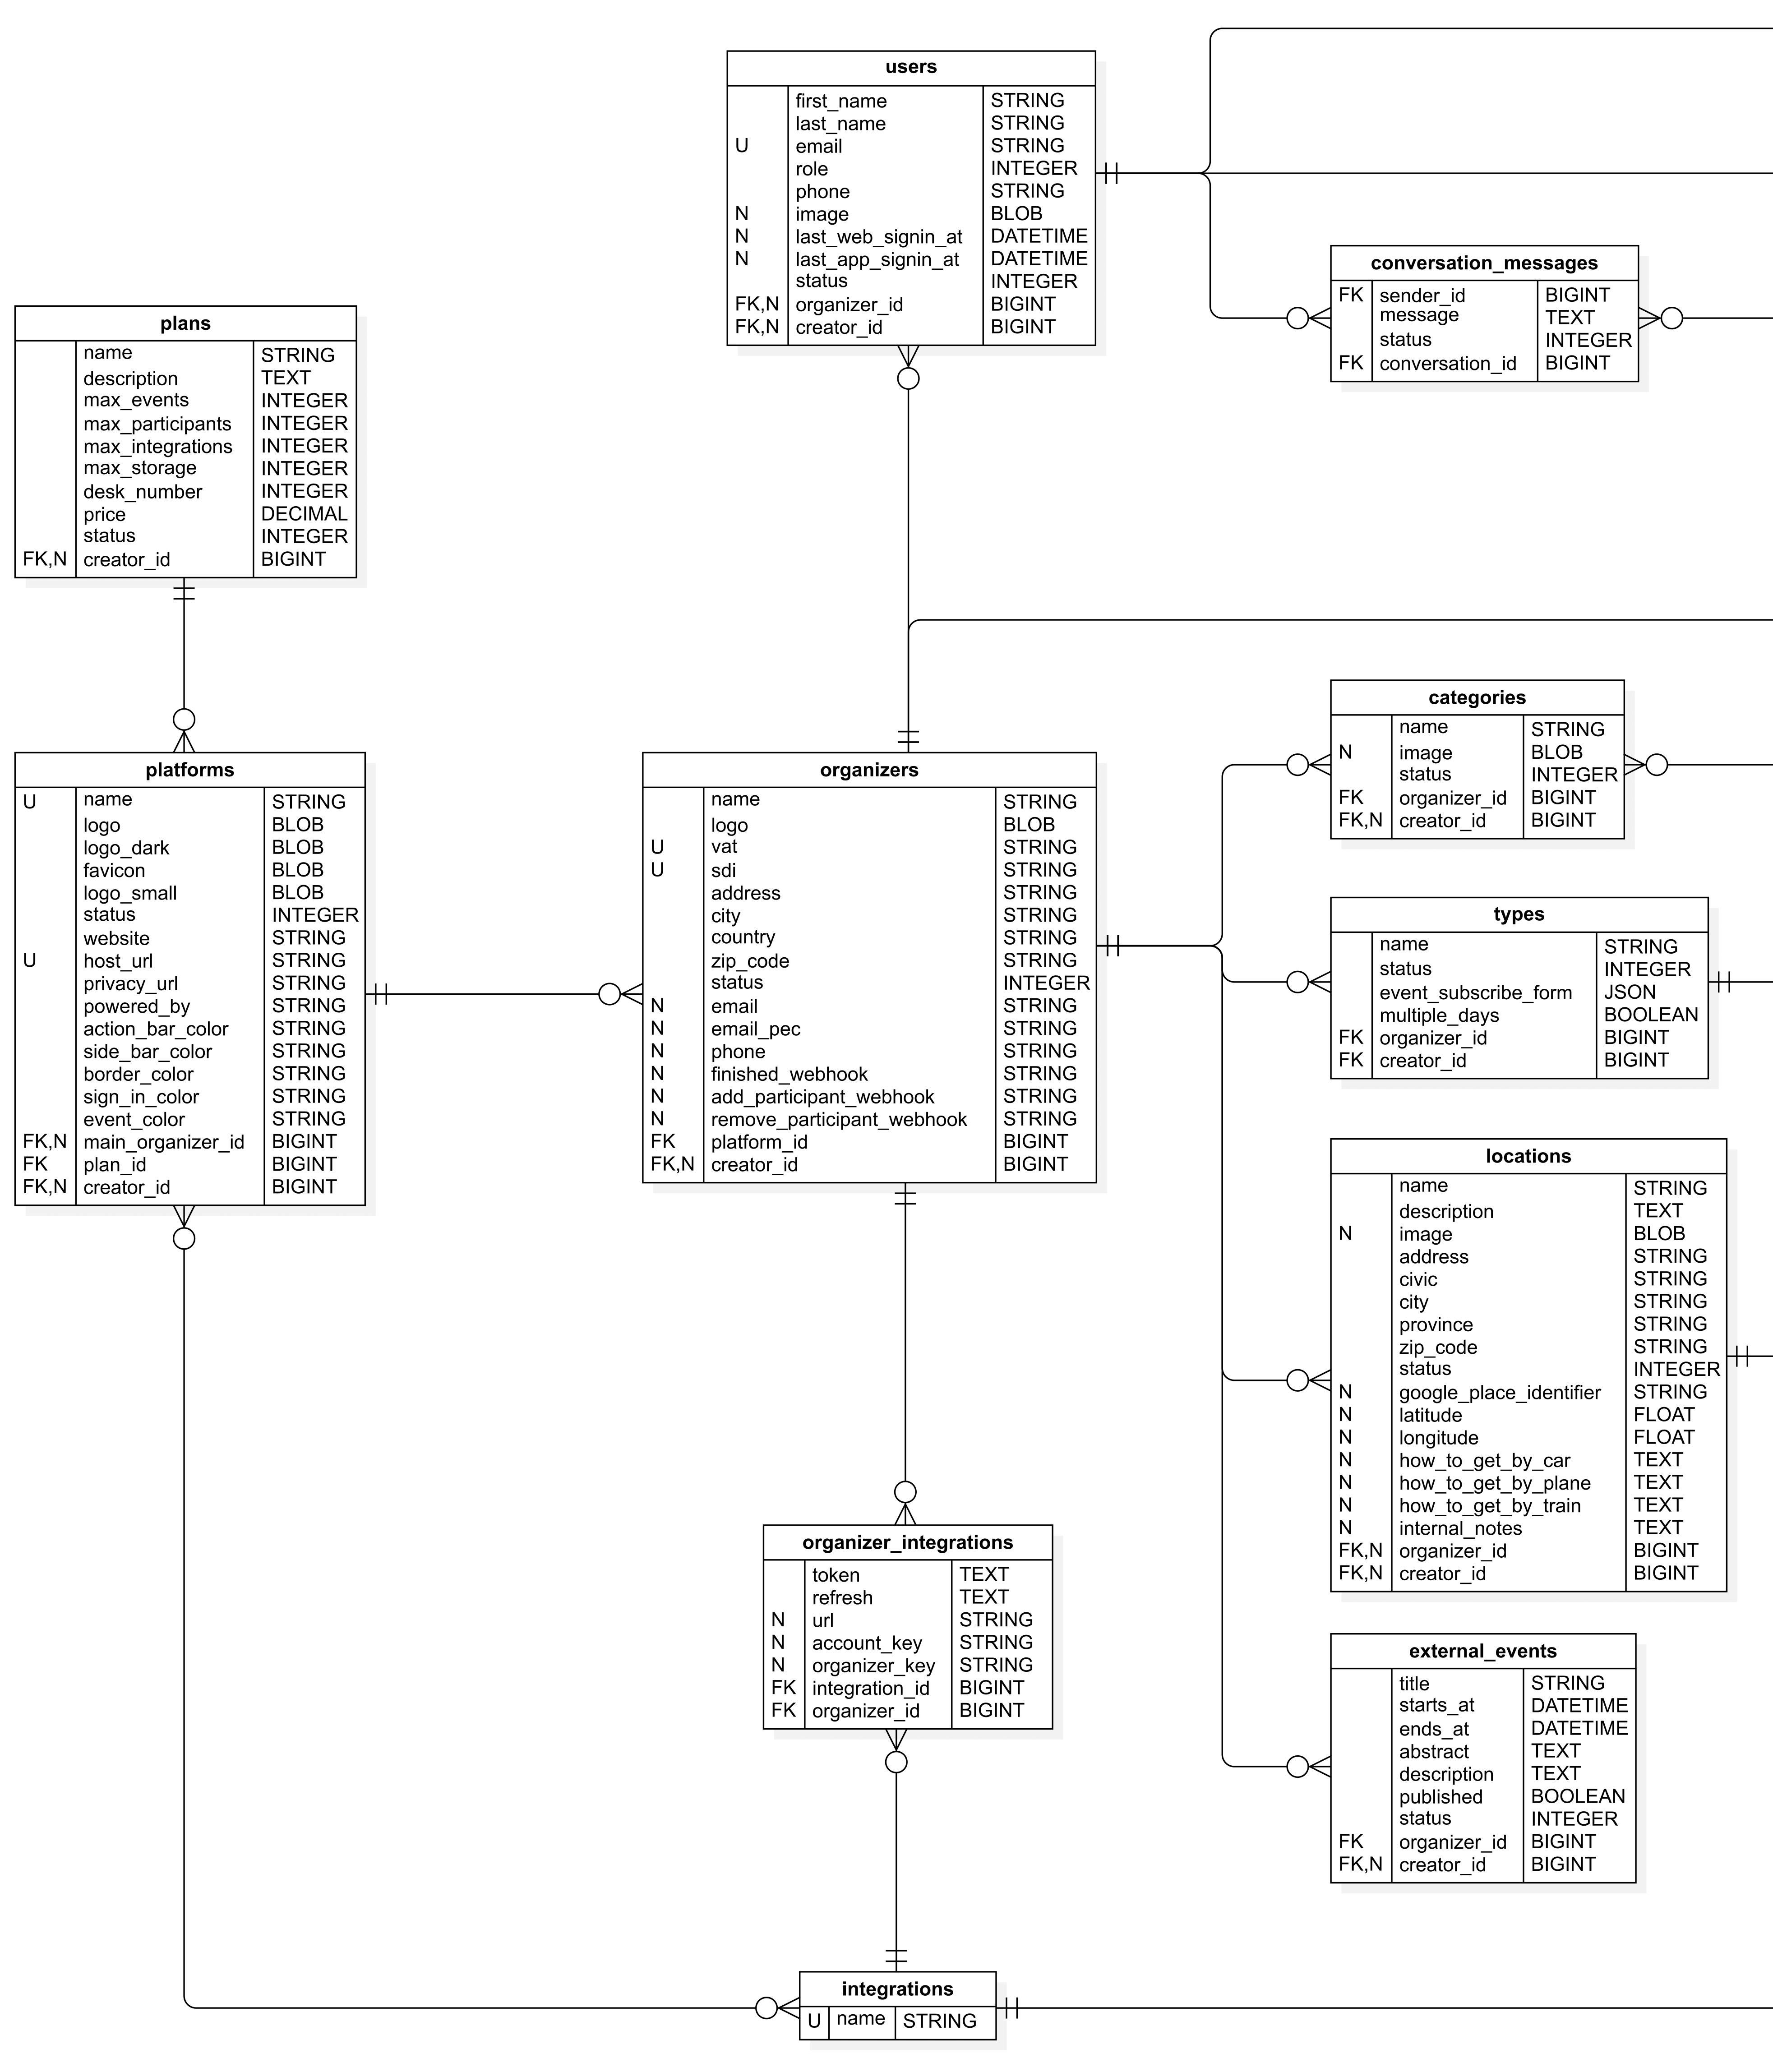
\includegraphics[width = \textwidth]{db/ER-west}
%	\caption{Sezione sinistra del dettaglio del diagramma ER}
%	\label{fig:er-west}
%\end{figure}
%
%\begin{figure}[b]
%	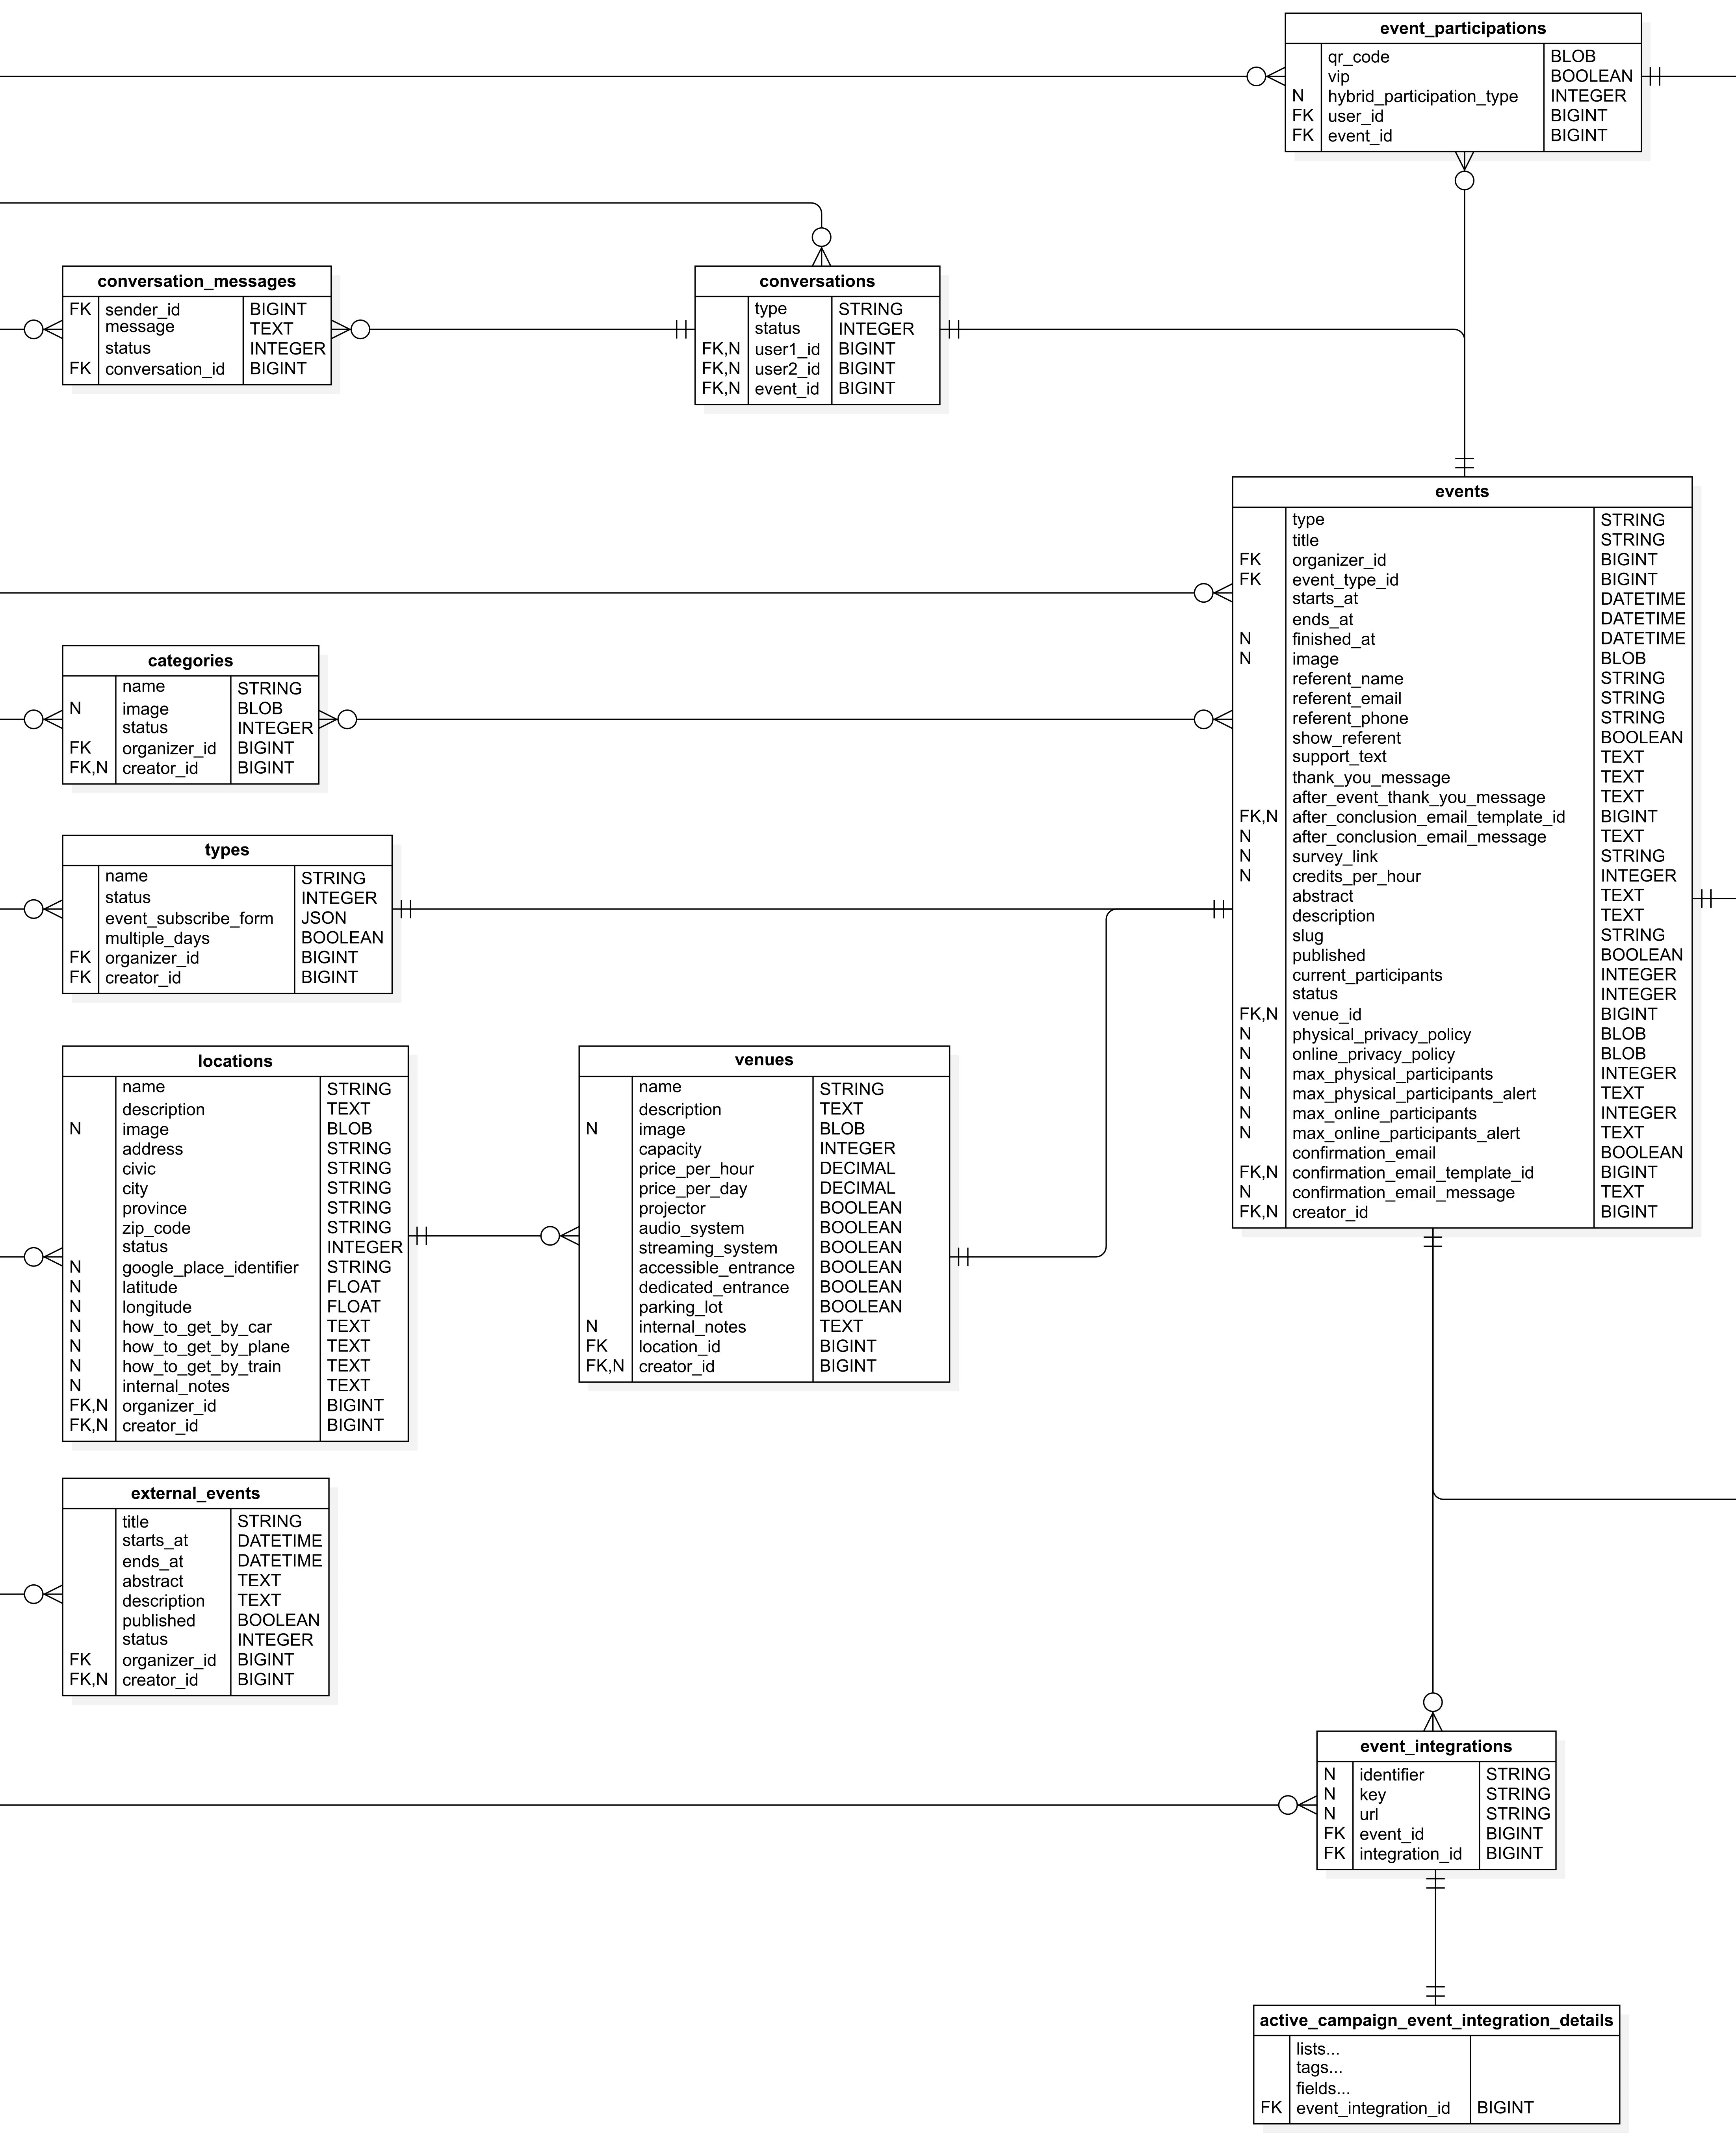
\includegraphics[width = \textwidth]{db/ER-center}
%	\caption{Sezione centrale del dettaglio del diagramma ER}
%	\label{fig:er-center}
%\end{figure}
%
%\begin{figure}[b]
%	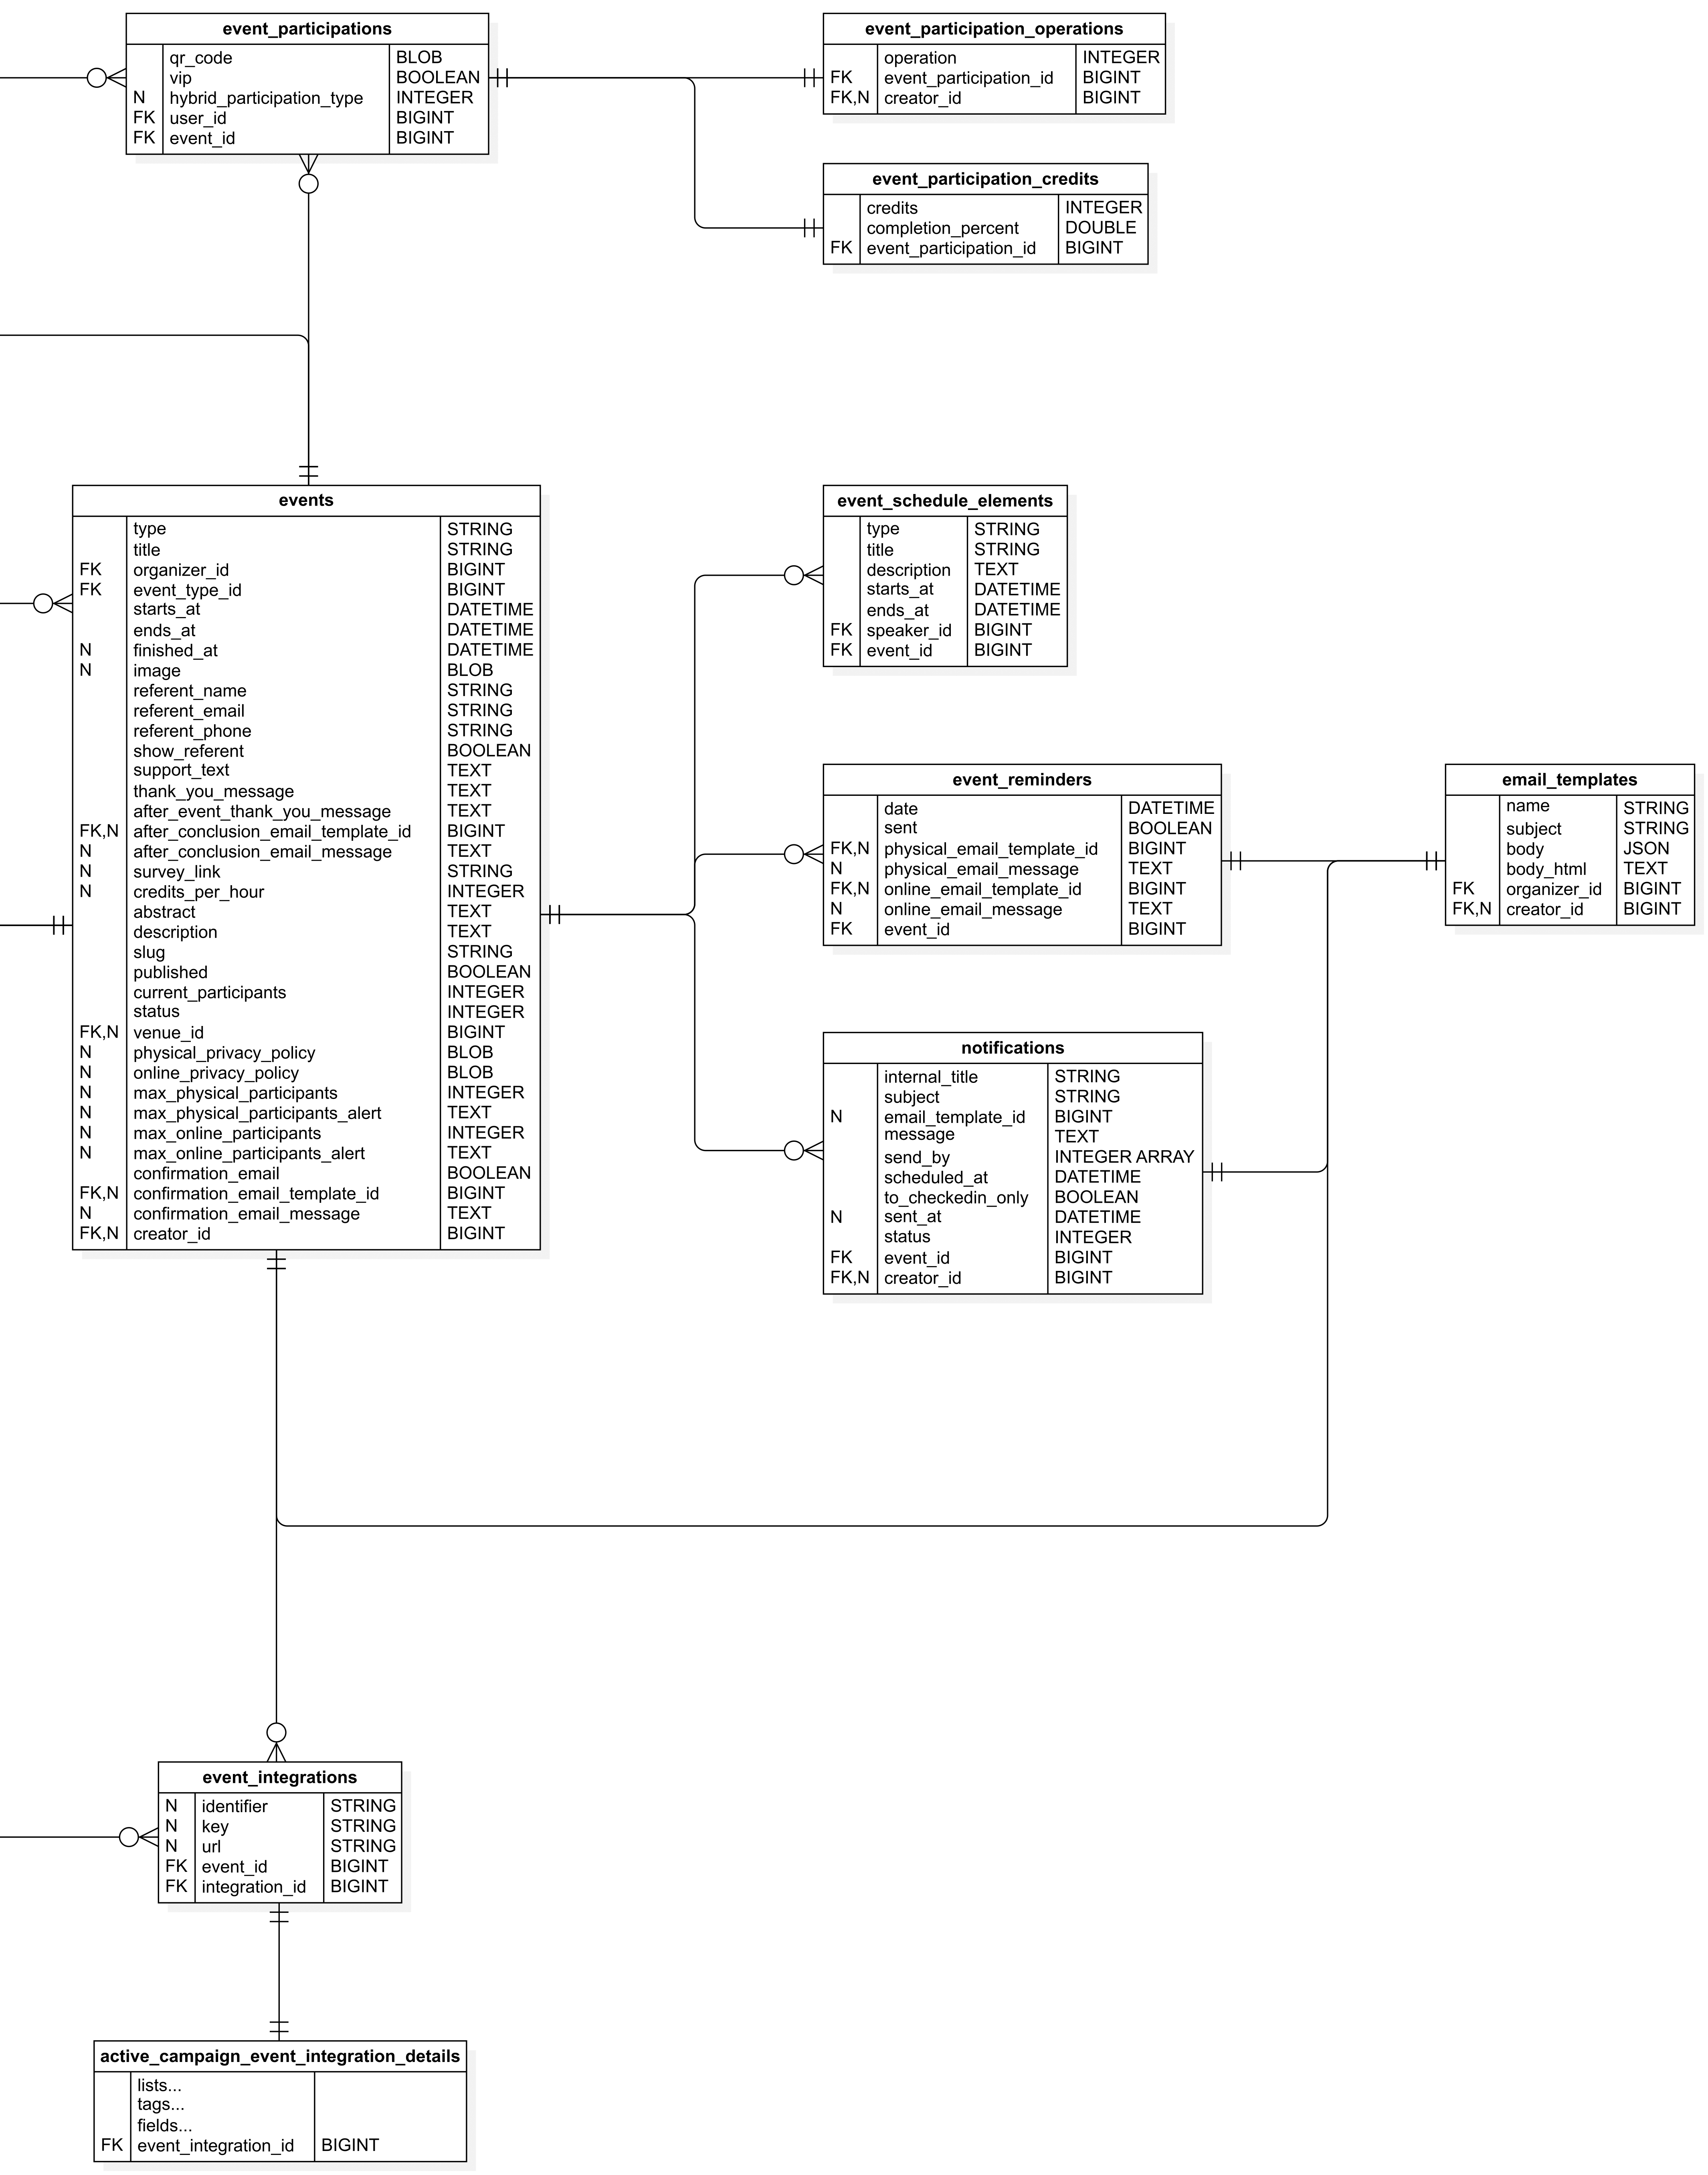
\includegraphics[width = \textwidth]{db/ER-east}
%	\caption{Sezione destra del dettaglio del diagramma ER}
%	\label{fig:er-east}
%\end{figure}

  
  \appendix

  % Materiale finale
  \backmatter
  % !TEX encoding = UTF-8
% !TEX TS-program = pdflatex
% !TEX root = ../tesi.tex

%**************************************************************
% Bibliografia
%**************************************************************

\cleardoublepage
\chapter{Bibliografia}

\nocite{*}
% Stampa i riferimenti bibliografici
\printbibliography[heading=subbibliography,title={Riferimenti bibliografici},type=book]

% Stampa i siti web consultati
\printbibliography[heading=subbibliography,title={Siti web consultati},type=online]


\end{document}
